\documentclass[tikz,border=2pt]{standalone}
\usepackage{tikz,pgfplots,pgf}
\usepackage{ifthen}
\begin{document}
\newcommand{\q}{0}
\newcommand{\w}{3}

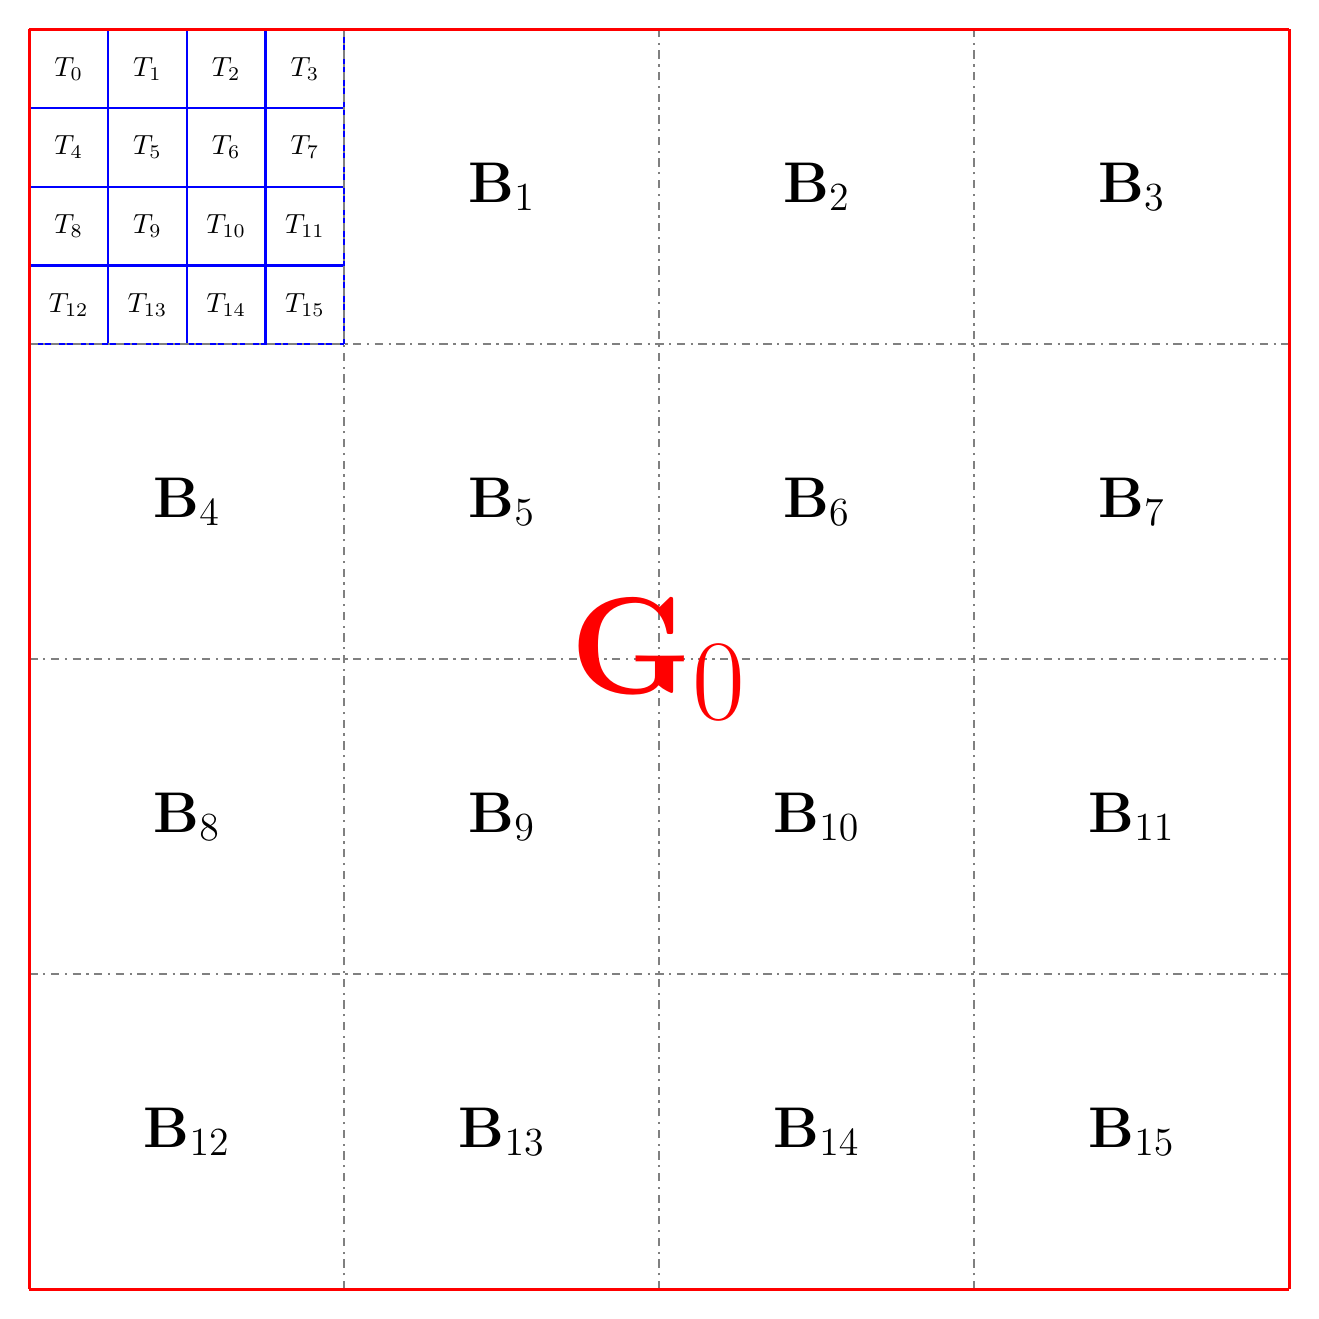
\begin{tikzpicture}
    %\draw[step=1cm, gray, thin,dashed] (0,0) grid (16,16);
    \draw[step=1cm, blue, thick] (0,12) grid (4,16);
    \draw[step=4cm, gray, thick,dashdotted] (0,0) grid (16,16);
    %\draw[step=4cm, green,  thick, loosely dashed] (0,0) grid (4,4);
    \draw[step=16cm, red, very thick] (0,0) grid (16,16);


    \foreach \x in {3,...,0}
    {
    \foreach \y in {3,...,0}
      {
        \node (\x\y) at (\x+0.5, 15-\y+0.5) {$T_{\pgfmathparse{int(abs(\x + 4*\y))}\pgfmathresult}$};

         \ifthenelse{\NOT 0 = \x \OR \NOT 3 = \y}{\node (b\x\y) at ({(4*\x)+2}, {(4*abs(\y)+2)}) { \huge $\mathbf{B}_{\pgfmathparse{int(abs(12-4*\y+\x))}\pgfmathresult}$};}{}

      }
    }
    \node[scale=2] (b00) at (8, 8) {\Huge \color{red} $\mathbf{G}_{0}$};



\end{tikzpicture}

\end{document}
